\section{Overview}
\label{overview}

This thesis is organized into a total of six chapters. In this chapter (Chapter 1), the motivations for carrying out this research were presented together with a brief overview of the objectives and research questions.

Chapter \ref{chap2} provides an overview of the foundational areas and concepts critical to this thesis. It outlines the fields of XAI which are related to the gaps this thesis aims to fill. Furthermore, an overview of EDM and its intersection with XAI is provided, in addition to the formal definitions of techniques frequently cited throughout the thesis. 

Chapters \ref{chap:AssALE} and \ref{chapter4} present the main contributions of this thesis. Chapter 3 formally delineates how different strategies to handle the data relationships affect post-hoc XAI techniques. It further empirically demonstrates the robustness of ALE in recovering the true effects of features in comparison with other techniques on different data dependence scenarios. 

Motivated by the results of Chapter \ref{chap:AssALE}, Chapter \ref{chapter4} subsequently introduces ALE-based metrics for assessing feature effect size. Each chapter begins with an introduction section that provides the necessary context and motivation, along with a brief review of related works that are specific to the chapter’s individual contribution. This structure results in a smoother overlap between chapter introductions, which, while not ideal, is necessary to ensure clarity and better position its contributions to the literature. The chapters also detail the methodology, experiments, and results of each contribution. 

Chapter \ref{chap: realApplication} showcases the usefulness of the ALE-based metrics developed in Chapter \ref{chapter4} to a practical case study. It presents a data-mining solution to investigate what and how variables have impacted Brazilian secondary school performance over a period of 11 years. 

Finally, Chapter \ref{chap: conclusion} presents the concluding remarks and discusses the main contributions of this thesis, and directions are outlined for possible future research.

Figure \ref{fig:thesis_flow} depicts the overview of this thesis through a diagram. The diagram, delineated by a blue box, illustrates the direct correlation between specific chapters of the thesis and their corresponding scientific publications, highlighting the integration of these publications into the thesis discourse. In contrast, the gray box encapsulates additional publications that, while not directly tied to individual thesis chapters, fall within the broader scope of the thesis topic - extract knowledge from educational data using ML. Notably, all publications presented are authored with the thesis candidate as the first author in the Ph.D. period.

\begin{figure}[ht!]
\centering
\caption{\textmd{Overview of Thesis Structure and Related Publications: Publications directly related to thesis chapters are shown in blue boxes, while additional publications within the thesis topic are in gray boxes. All works are first-authored}}
\label{fig:thesis_flow}
\fcolorbox{gray}{white}{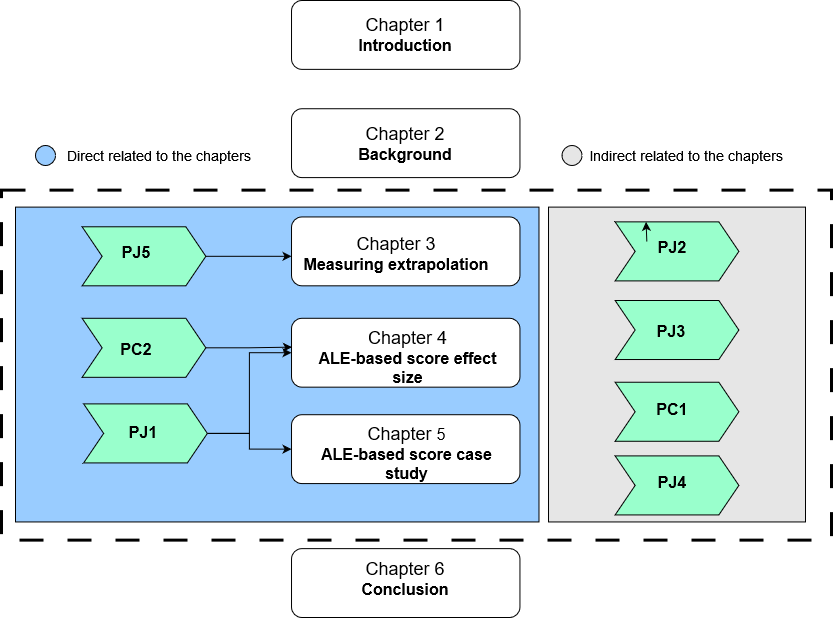
\includegraphics[width=0.7\textwidth]{images/captitulo1/Flow_thesis_diagram_researchers_chapters.drawio.png}}
\par\medskip\ABNTEXfontereduzida\selectfont\textbf{Source: self-provided}  
\par\medskip
\end{figure}